%% ----------------------------------------------------------------
%% Results.tex
%% ---------------------------------------------------------------- 
\chapter{Results and Discussion} \label{Chapter:Results}

\section{VGG Architecture Comparisons}
To estimate the impact of the backbone's depth and the side-network's architecture, each RetinaNet proposed architecture gets deployed on each VGG network separately. \fref{ch5:fig1} and \ref{ch5:fig2} show how AP and F1-score scale with the depth of the backbone network.   

\begin{figure}[!htb]
  \centering
  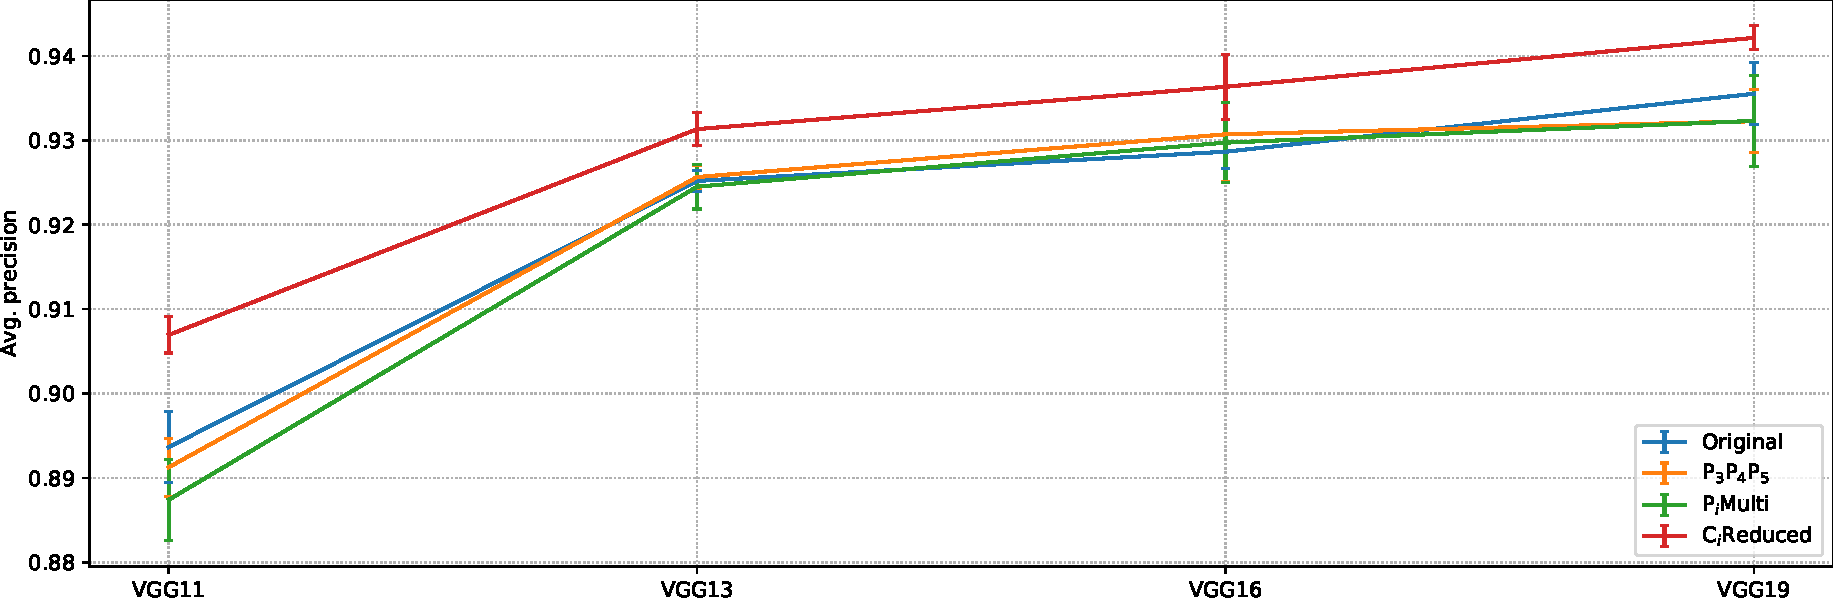
\includegraphics[width=\textwidth]{figures/ch5/fig1.pdf}
  \caption{Comparative results of Avg. Precision versus the four VGG models, for each proposed RetinaNet model. Results are averaged over 10 times.}
  \label{ch5:fig1}
\end{figure}

\begin{table}[!htb]
  \centering
  \resizebox{0.75\textwidth}{!}{
  \begin{tabular}{ccccc}
  \toprule
  \textbf{Avg. Precision} & \textbf{VGG11} & \textbf{VGG13} & \textbf{VGG16} & \textbf{VGG19} \\
  \midrule
  Original (202)								&	0.894$\pm$0.004		&	0.925$\pm$0.001		& 	0.929$\pm$0.002		&	0.936$\pm$0.004\\
  $\text{P}_3\text{P}_4\text{P}_5$ (202) 			&	0.891$\pm$0.003		&	0.926$\pm$0.001		& 	0.931$\pm$0.006		&	0.932$\pm$0.004\\
  $\text{P}_\text{i}\text{Multi}$ (202)				&	0.887$\pm$0.005		&	0.925$\pm$0.003 		& 	0.930$\pm$0.005		&	0.932$\pm$0.005\\
  \textbf{$\text{C}_\text{i}\text{Reduced}$} (202) 	&	\textbf{0.907$\pm$0.002}	&	\textbf{0.931$\pm$0.002} 	&	\textbf{0.936$\pm$0.004}	&	\textbf{0.942$\pm$0.001}\\
  \bottomrule
  \end{tabular}
  }
  \caption{Indicative values of the Avg. Precision for the selected four VGG models, for each proposed RetinaNet model (\fref{ch5:fig1}). Parentheses indicate the input resolution.}
  \label{ch5:tab1}
\end{table}

From \fref{ch5:fig1}, it can be seen that the average precision scales with the depth of the network steadily. The increment rate is not large enough to warrant exploring deeper models, as the number of parameters and training time increases adversely. The average precision versus depth diagram shows that indeed, the depth of VGG helps the model detecting more relevant objects.

However, the F1-score as shown in \fref{ch5:fig2}, does not follow this trend, as it reaches its climax under VGG16 for the $\text{P}_\text{i}\text{Multi}$ and $\text{C}_\text{i}\text{Reduced}$ models, while the Original model exhibits a slight increase.
F1-score, after VGG16, illustrates that neither the depth of the model nor the side-network deployment can confine the model from predicting false positives.

\begin{figure}[!htb]
  \centering
  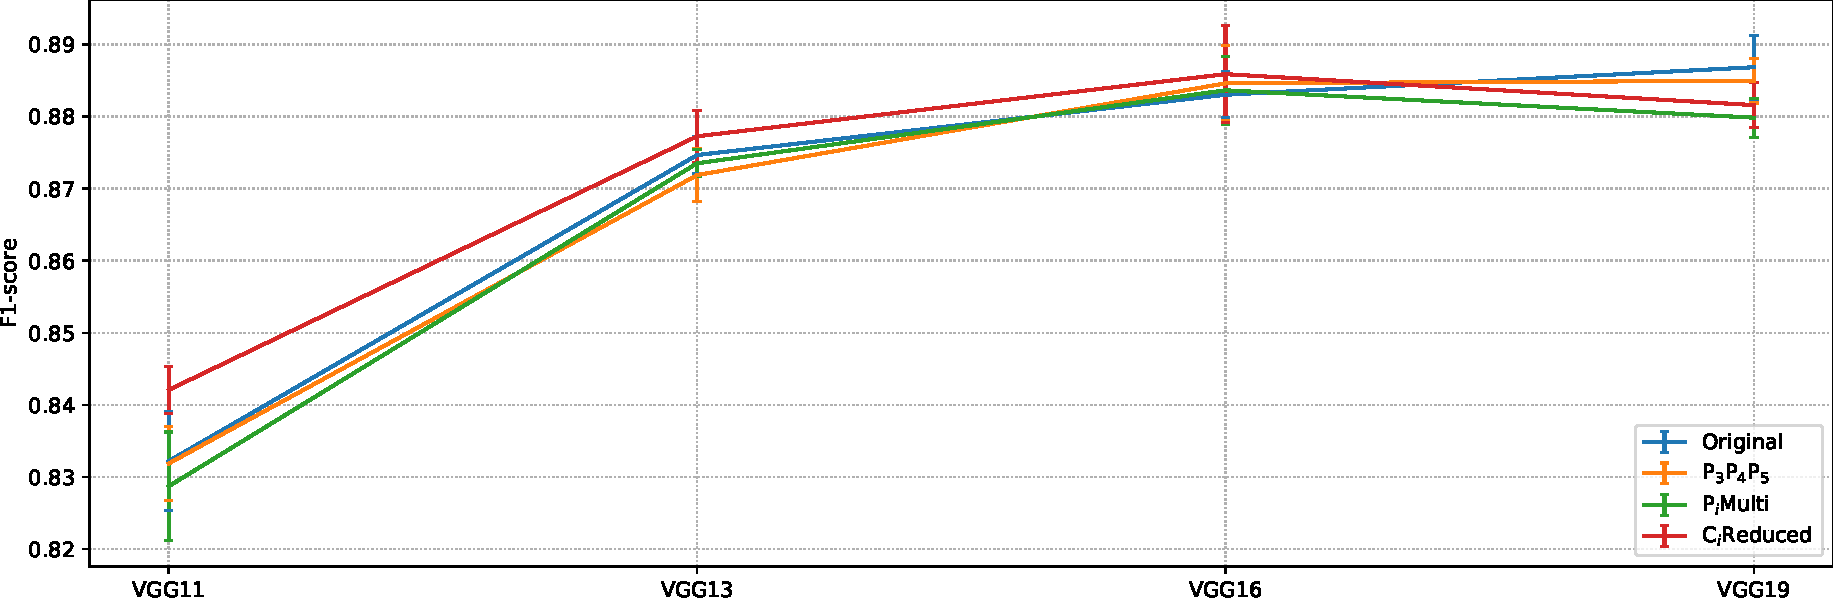
\includegraphics[width=\textwidth]{figures/ch5/fig2.pdf}
  \caption{Comparative results of the F1-score versus the four VGG models, for each proposed RetinaNet model. Results are averaged over 10 times.}
  \label{ch5:fig2}
\end{figure}

\begin{table}[!htb]
  \centering
  \resizebox{0.75\textwidth}{!}{
  \begin{tabular}{ccccc}
  \toprule
  \textbf{F1-score} & \textbf{VGG11} & \textbf{VGG13} & \textbf{VGG16} & \textbf{VGG19} \\
  \midrule
  Original (202)							&	0.832$\pm$0.007		&	0.875$\pm$0.003		& 	0.883$\pm$0.003	&	\textbf{0.887$\pm$0.004}\\
  $\text{P}_3\text{P}_4\text{P}_5$ (202)		&	0.832$\pm$0.005		&	0.872$\pm$0.004		& 	0.885$\pm$0.005	&	0.885$\pm$0.003\\
  $\text{P}_\text{i}\text{Multi}$ (202)			&	0.829$\pm$0.008		&	0.874$\pm$0.002 		& 	0.884$\pm$0.005	&	0.880$\pm$0.003\\
  \textbf{$\text{C}_\text{i}\text{Reduced}$} (202) &	\textbf{0.842$\pm$0.003}	&	\textbf{0.877$\pm$0.004}	&	\textbf{0.886$\pm$0.007}	&	0.882$\pm$0.003\\
  \bottomrule
  \end{tabular}
  }
  \caption{Indicative values of F1-score for the selected four VGG models, for each proposed RetinaNet model (\fref{ch5:fig2}). Parentheses indicate the input resolution.}
  \label{ch5:tab2}
\end{table}

Concerning the side-network, apart from $\text{C}_\text{i}\text{Reduced}$, the rest RetinaNet deployments did not demonstrate any striking difference. Particularly, the Original and the $\text{P}_3\text{P}_4\text{P}_5$ deployments performed similarly, confirming the prior speculations about layer redundancy. $\text{P}_3\text{P}_4\text{P}_5$ achieved almost the same accuracy with a 10 FPS gain in inference time. $\text{P}_\text{i}\text{Multi}$ demonstrated that separate sub-network heads did not influence performance, but surprisingly, the excessive parameters had minor impact on the inference time. Under most VGG depths, $\text{C}_\text{i}\text{Reduced}$ outperformed notably the rest of the architectures, especially in AP. \textbf{This observation manifests that the problem under study is not affected considerably by the complexity of the side-network in ways such as: integrating high-level semantic feature maps, attaching separate classifier-regressor heads or increasing the depth.} Nonetheless, a lighter version of the original RetinaNet, inspired by the SSD pipeline, addresses the apple detection problem through the ACFR dataset satisfactorily.

\tref{ch5:tab3} shows that inference time scales with the depth of the model upon increasing the total parameters, apart from the VGG16 and VGG19, which have the same inference time. Lightweight RetinaNet - $\text{C}_\text{i}\text{Reduced}$, as expected, holds the highest detection rates among the rest models.

\begin{table}[!htb]
  \centering
  \resizebox{0.8\textwidth}{!}{
  \begin{tabular}{ccccc}
  \toprule
  \textbf{Inference time (FPS)}	  			& \textbf{VGG11} 	& \textbf{VGG13} 	& \textbf{VGG16} 	& \textbf{VGG19} \\
  \midrule
  Original (202)							&	61.0$\pm$3.5		&	58.8$\pm$3.0		& 	55.3$\pm$2.5	&	55.3$\pm$2.5\\
  $\text{P}_3\text{P}_4\text{P}_5$ (202) 		&	71.1$\pm$3.3		&	69.1$\pm$2.5		& 	67.3$\pm$2.0	&	67.3$\pm$2.0\\
  $\text{P}_\text{i}\text{Multi}$ (202)			&	67.8$\pm$4.4		&	67.3$\pm$3.1		& 	65.2$\pm$2.7	&	65.2$\pm$2.7\\
  \textbf{$\text{C}_\text{i}\text{Reduced}$} (202)	& \textbf{74.0$\pm$5.1}	& \textbf{71.1$\pm$4.5}	& \textbf{65.2$\pm$4.3} 	& \textbf{65.2$\pm$4.3}\\
  \bottomrule
  \end{tabular}
  }
  \caption{Inference time for every VGG. Detection rates depend heavily on the No. of parameters of the model and the input resolution. However, the transition from VGG16 to VGG19 did not show any change.}
  \label{ch5:tab3}
\end{table}

All VGG models were initialised upon the pre-trained ImageNet weights. Training with random weight initialisation delayed convergence but did not show any improvement in the results, as demonstrated in \cite{bargoti2017deep}. Transfer learning between the VGG models, that is transferring the weights progressively from VGG11 to VGG19 (\cite{simonyan2014very}), did not show any other improvement in performance rather than saving training from a couple of epochs ($\sim3$ minutes with a resolution of $202\times308$).


\section{Performance - Training Size Relation}\label{size_relation}

This section presents a performance analysis of RetinaNet - $\text{C}_\text{i}\text{Reduced}$ (202)	over the size of the training dataset. For each training subset, N samples were drawn from the training dataset randomly, without replacement (negative samples were discarded). 

 \begin{figure}[!htb]
  \centering
  \subfigure[]{
    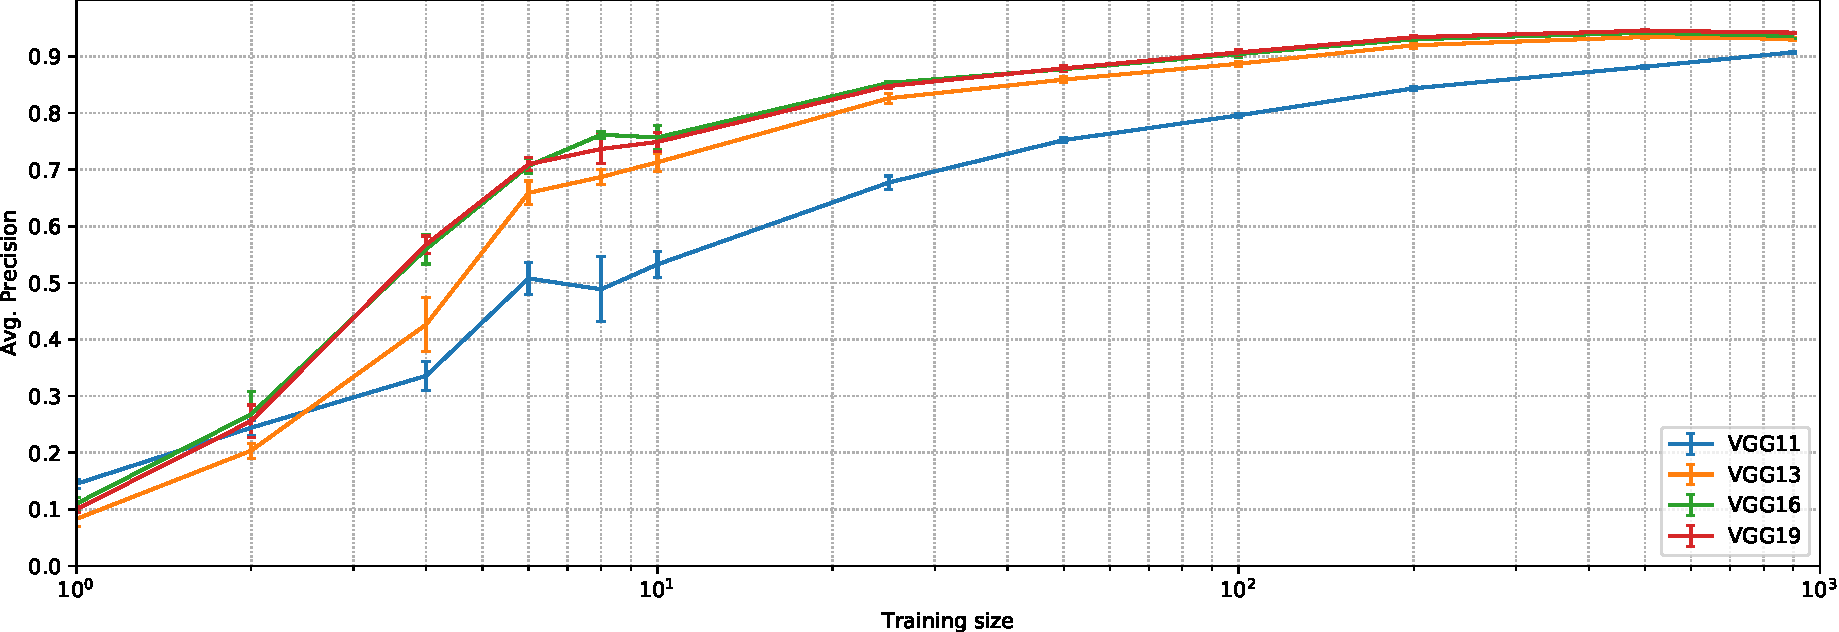
\includegraphics[width=0.9\textwidth]{figures/ch5/fig3_1.pdf}
    \label{ch5:fig3_1}
  }
  \subfigure[]{
    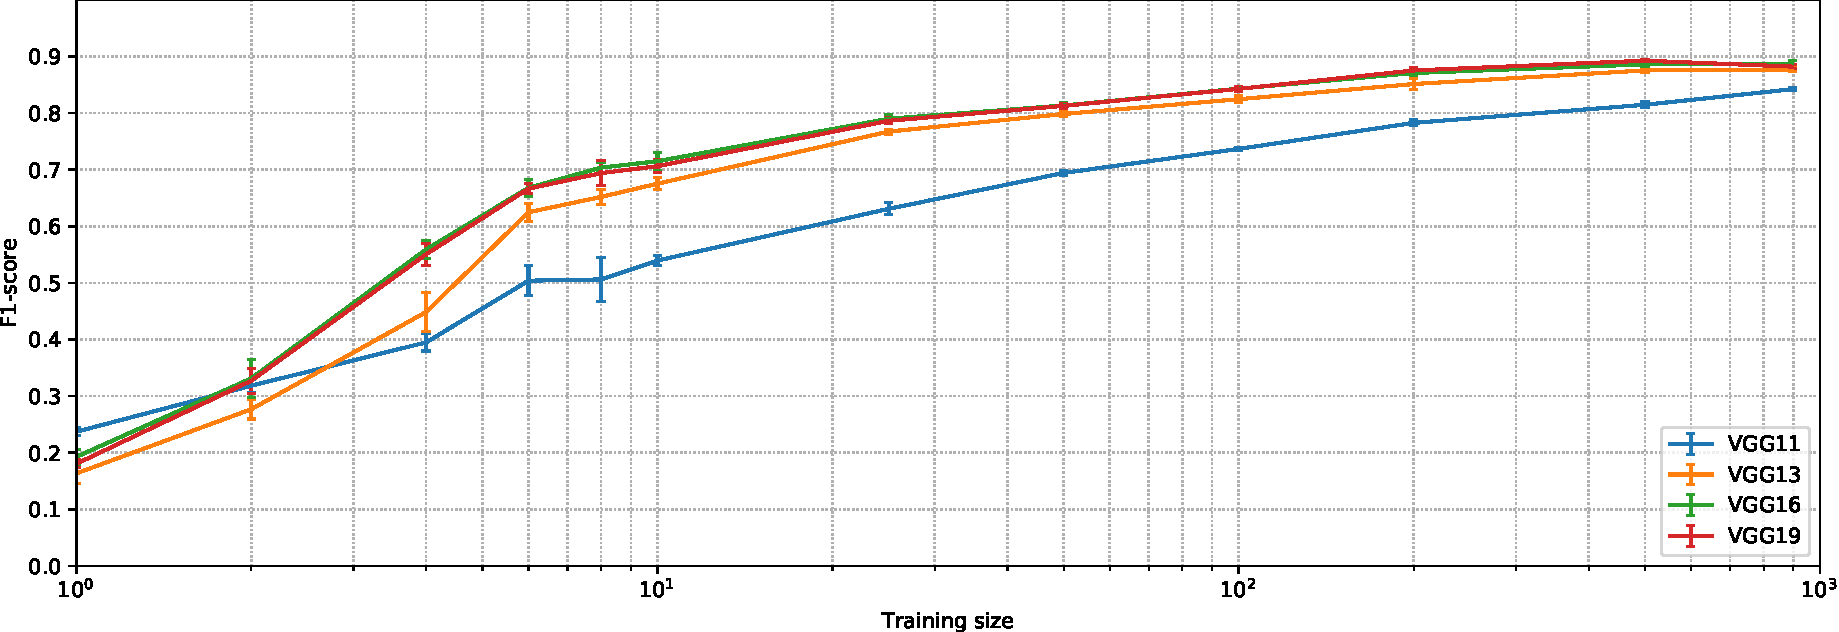
\includegraphics[width=0.9\textwidth]{figures/ch5/fig3_2.pdf}
    \label{ch5:fig3_2}
  }
  \caption{Avg. Precision and F1-score as a function of the number of training images on RetinaNet - $\text{C}_\text{i}\text{Reduced}$ (202), for each VGG network.}
  \label{ch5:fig3}
\end{figure}

The subsets were created once and then used for 10 training sessions each. The models were prone to overfitting, particularly those trained on small datasets; thus, early stopping was implemented to obtain the maximum possible performance. \fref{ch5:fig3} makes evident that the model performs competently already from the first 10 samples. Furthermore, 200 to 500 samples are enough to achieve state-of-the-art performance. From the first 6 samples, RetinaNet outperforms Faster R-CNN in the work of \cite{bargoti2017deep} by 0.1 in every consecutive training subset.



Regarding the backbone's network depth, VGG16 and VGG19 show their superiority over the rest architectures consistently. Another interesting feature of \fref{ch5:fig3} is that in training sessions consisting more than 10 samples, VGG11 attained the same performance with VGG16-19 only by decupling the dataset.

\section{Peak Detection and Evaluation}
To obtain maximum performance, RetinaNet - $\text{C}_\text{i}\text{Reduced}$ was trained on VGG16, using three resolutions ($202\times308$, $512\times781$ and $800\times1220$) as described in \sref{training_details}, with F1-score being the primary evaluation metric. Models presented here were trained initially on the training dataset, and then both on the training and validation dataset, while being evaluated on the held-out testing dataset.

\tref{ch5:tab4} shows that performance increases with resolution, with the best model achieving a maximum F1-score of \textbf{0.907}, outperforming the previous state-of-the-art model (\cite{bargoti2017deep}). \cite{liang2018apple} gave more emphasis on real-time detection achieving $\sim$44 FPS using the SSD(300), while RetinaNet - $\text{C}_\text{i}\text{Reduced}$ (VGG16)[202] attains a detection rate of $\sim$70 FPS outperforming both of their models. RetinaNet - $\text{C}_\text{i}\text{Reduced}$(VGG16), beaten SSD in performance and inference time by using even smaller resolution. A resolution of 800 improved performance, in terms of F1-score by $\sim1\%$, but with a considerable increase in training time versus the smaller resolution of 202. Specifically, the models trained on the original image dimensions ($202\times308$), required x4 times less time to train in comparison to the ones that used ($800\times1220$) and also, they had x5.5 times less inference time (65.2 FPS vs 12.6FPS).
Moreover, from \tref{ch5:tab4} it can be seen that, while the IoU threshold was set equal to 0.2, as in the previous sections, the mean IoU between ground truths and predictions is quite high, making very accurate localisations.

\begin{savenotes}
\begin{table}[!htb]
  \centering
  \resizebox{0.8\textwidth}{!}{
  \begin{tabular}{ccccc}
  \toprule
  \textbf{Training set and resolution}	& \textbf{AP} 	& \textbf{F1} 	& \textbf{mIoU} 	&  \textbf{$\Delta E$} \\
  \midrule
  train. (202)					&	0.948	&	0.895		& 	0.793	&	0.099\\
  train. (512) 					&	0.953	&	0.903		& 	0.814	&	0.040\\
  train. (800)					&	0.952	&	0.903		& 	0.829	&	\textbf{0.016}\\
  train. + val. (202)				&	0.949	&	0.895		& 	0.807	&	0.081\\
  train. + val. (512)				&	0.954	&	0.905		& 	0.824	&	0.038\\
  train. + val. (800)				&	0.953	&	\textbf{0.907}	& 	0.835	&	0.025\\
  \midrule
  Faster R-CNN (ZF) [1]\footnote{[1]: \cite{bargoti2017deep}}		& 	-		&	0.892		&	-		&	-\\
  Faster R-CNN (VGG16) [1]								& 	-		&	0.904		&	-		&	-\\
  Faster R-CNN (VGG16) [2]\footnote{[2]: \cite{liang2018apple}}	& 	-		&	0.879		&	-		&	-\\
  \midrule
  SSD (300) [2]												& 	-		&	0.883		&	-		&	-\\
  SSD (500) [2]												& 	-		&	0.890		&	-		&	-\\
  \bottomrule
  \end{tabular}
  }
  \caption{Comparing performance of RetinaNet - $\text{C}_\text{i}\text{Reduced}$ (VGG16), trained on the training and on the combined training - validation set, with the state-of-the-art models. Parentheses indicate resolutions. Models were evaluated on $\text{IoU}_{th}=0.2$ and $\text{NMS}_{th}=0.3$.}
  \label{ch5:tab4}
\end{table}
\end{savenotes}

\begin{figure}[!htb]
  \centering
  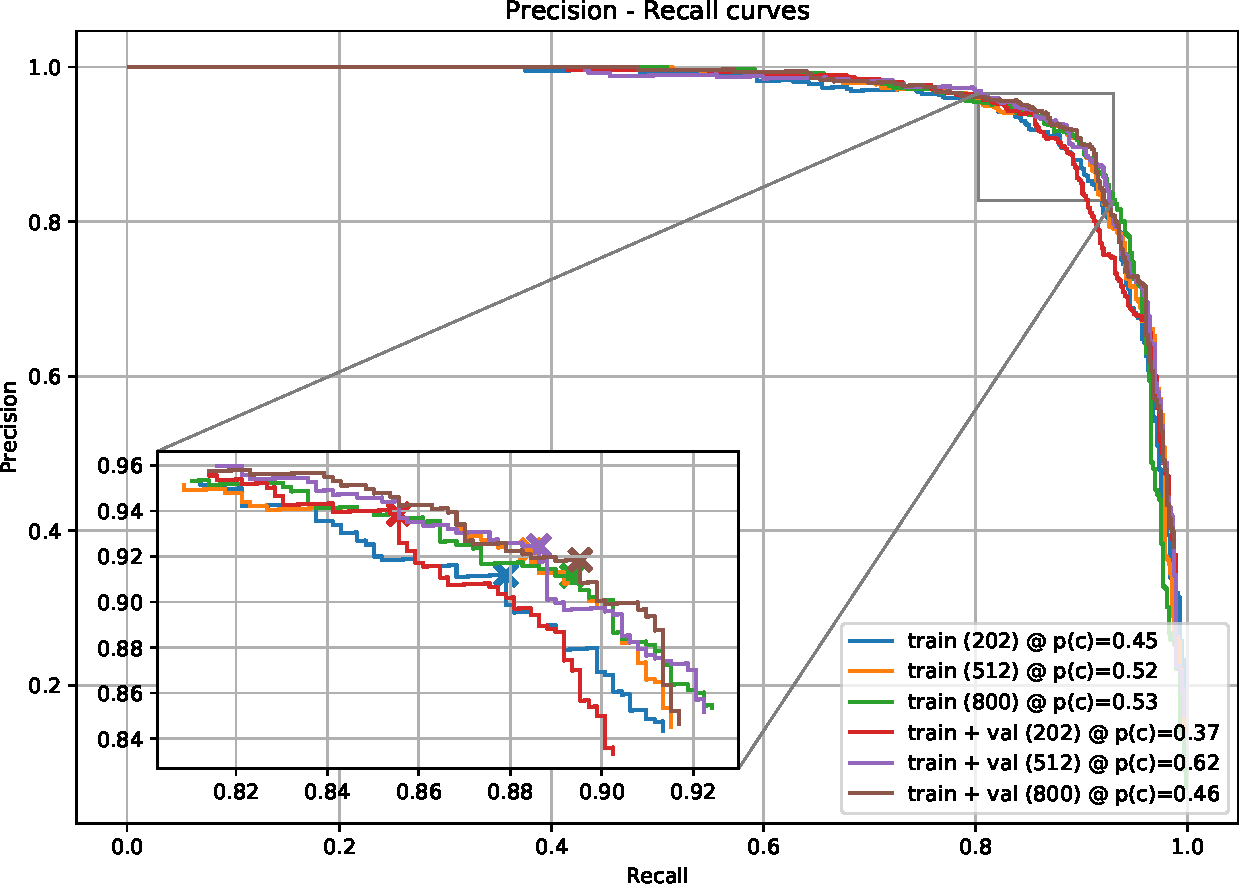
\includegraphics[width=0.6\textwidth]{figures/ch5/fig4.pdf}
  \caption{Precision - Recall curves for the RetinaNet - $\text{C}_\text{i}\text{Reduced}$ (VGG16). AP is defined by the area under the curve, while F1-score is the point on the curve where Precision and Recall take maximum values.}
  \label{ch5:fig4}
\end{figure} 

\fref{ch5:fig4} illustrates the precision-recall curves of the trained models presented in \tref{ch5:tab4}. All models maintain very high precision for all recall levels. Precision stays around 1.0 for most recall values and starts to drop after recall takes values higher than 0.8.

\subsection{Performance at Various IoU  and NMS Thresholds}\label{nms_threshold}
In most competitions such as in PASCAL-VOC, a prediction to be considered as positive needs at least an overlap of 0.5 with the ground truth. However, \cite{bargoti2017deep} state that an IoU threshold equal to 0.2 is sufficient for accurate fruit detection, eliminating the error cases where the localisation is imperfect. \fref{ch5:fig5_1} shows how the precision-recall curve changes under different IoU thresholds. The model maintains the same performance even under more strict settings such as raising the $\text{IoU}_{th}$ from 0.2 to 0.5. Only for $\text{IoU}_{th} \geq 0.8$, performance starts to degenerate.

 \begin{figure}[!htb]
  \centering
  \subfigure[]{
    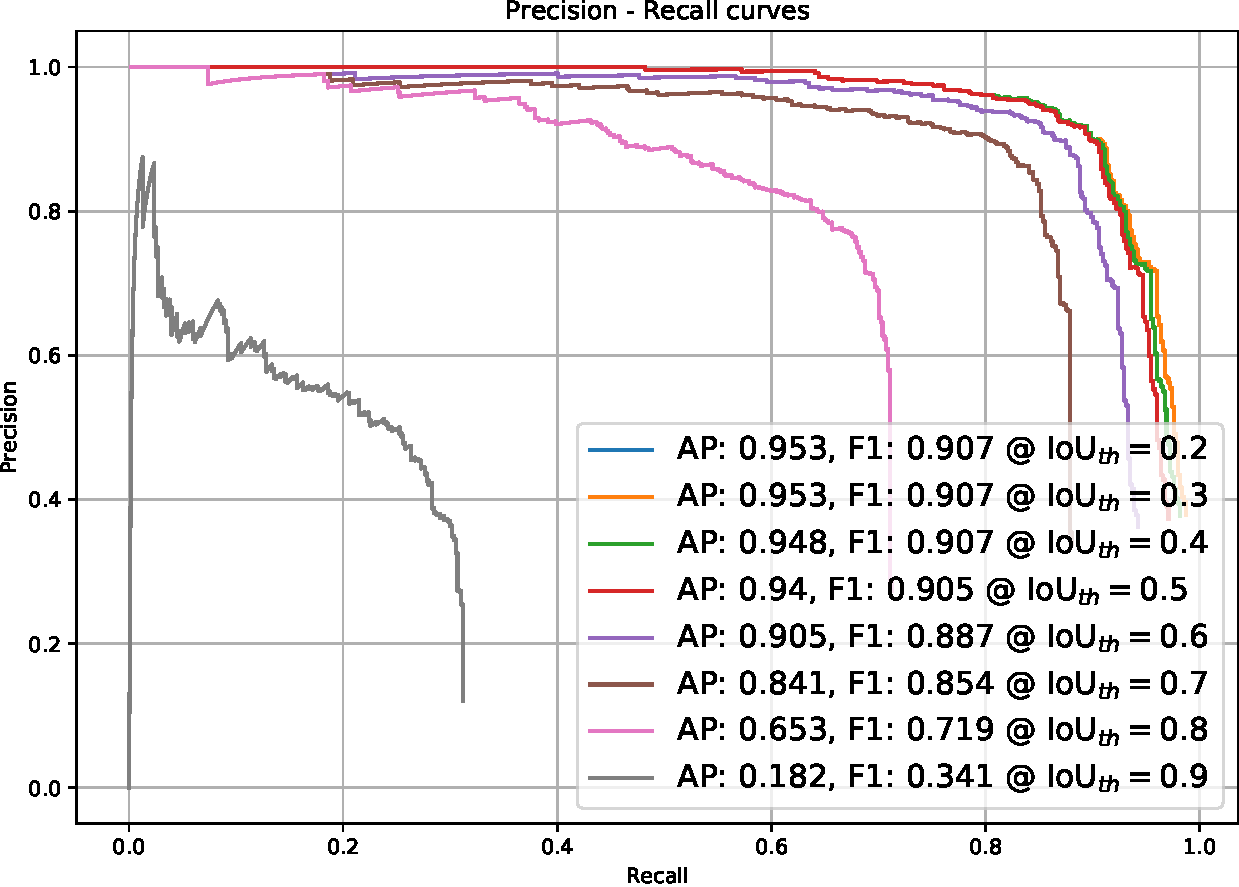
\includegraphics[width=0.45\textwidth]{figures/ch5/fig5_1.pdf}
    \label{ch5:fig5_1}
  }
  \subfigure[]{
    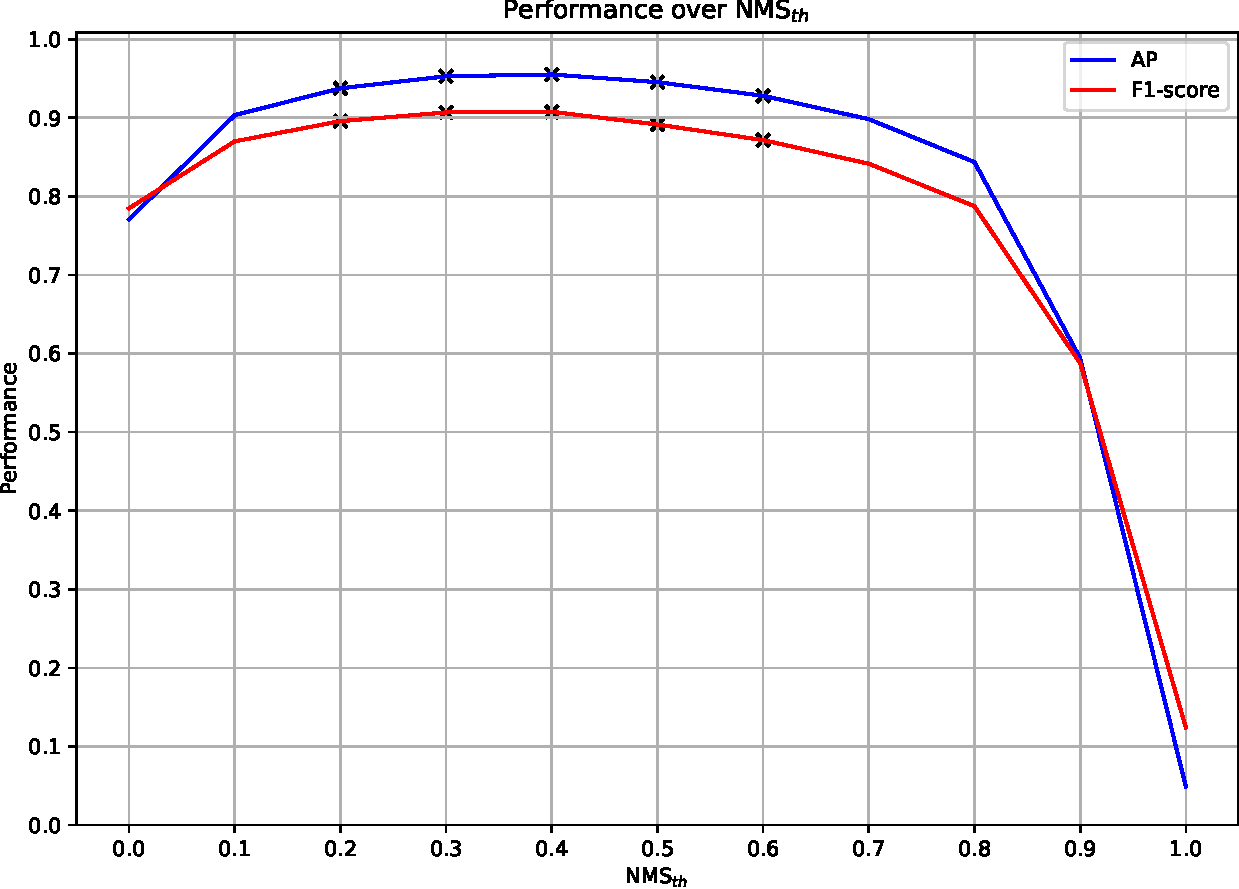
\includegraphics[width=0.45\textwidth]{figures/ch5/fig5_2.pdf}
    \label{ch5:fig5_2}
  }
  \caption{(a) Precision - Recall curves for the RetinaNet - $\text{C}_\text{i}\text{Reduced}$ (VGG16) under various $\text{IoU}_{th}$. Model's performance remains supreme even by increasing  $\text{IoU}_{th}$ from 0.2 to 0.5. (b) Performance over $\text{NMS}_{th}$. Performance is not very sensitive for $\text{NMS}_{th}$ between 0.2 and 0.6.}
  \label{ch5:fig5}
\end{figure}

\begin{table}[!htb]
  \centering
  \resizebox{0.5\textwidth}{!}{
  \begin{tabular}{cccccc}
  \toprule
  \textbf{$\text{NMS}_{th}$}	& \textbf{0.2} 	& \textbf{0.3}	& \textbf{0.4} 	& \textbf{0.5} 	& \textbf{0.6} 	\\
  \midrule
  \textbf{AP}				&	0.938	&	0.953	&	\textbf{0.955}	&	0.945	&	0.928	\\
  \textbf{F1-score}			&	0.896	&	0.907	&	\textbf{0.908}	&	0.891	&	0.872	\\	
  \bottomrule
  \end{tabular}
  }
  \caption{Indicative values of Avg. Precision and F1-score for selected $\text{NMS}_{th}$ at the default $\text{IoU}_{th}=0.2$. $\text{NMS}_{th}$ of 0.4 pushes performance a bit further.}
  \label{ch5:tab5}
\end{table}

\begin{figure}[!ht]
  \centering
  \subfigure[$\text{NMS}_{th}=0.3$]{
    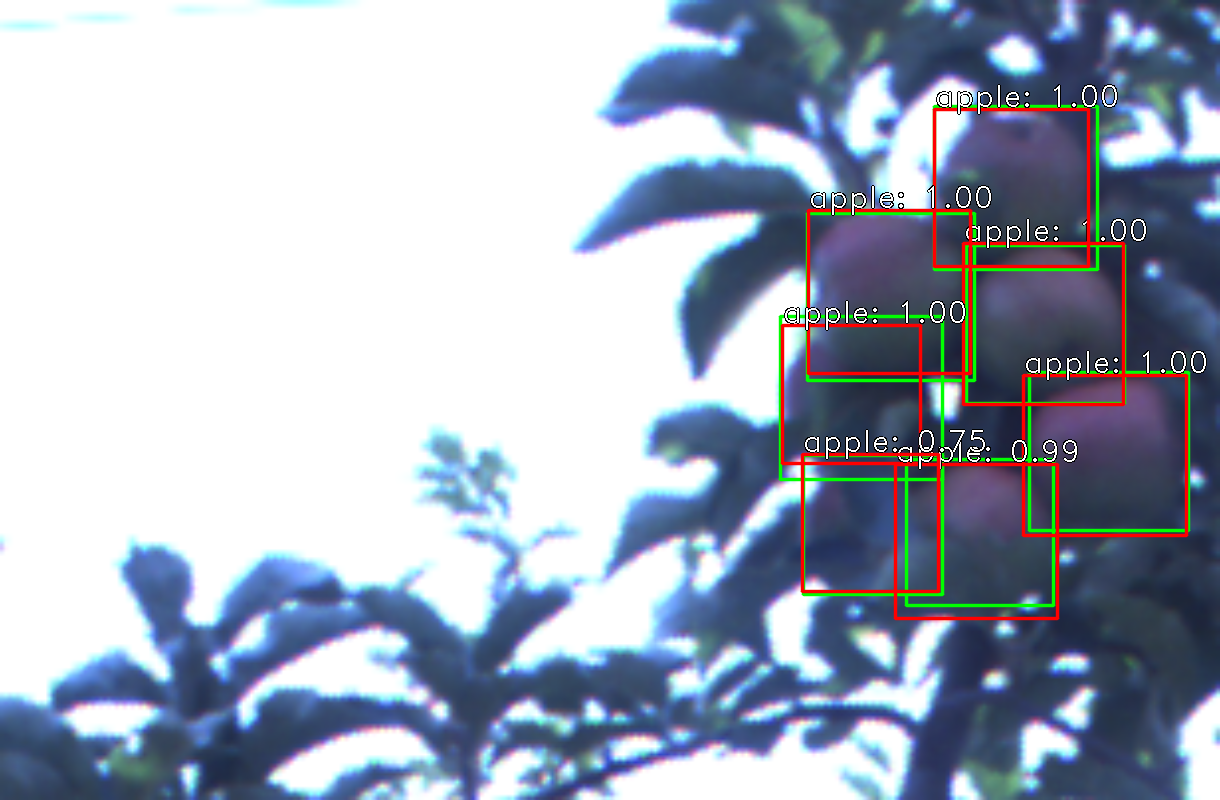
\includegraphics[width=0.38\textwidth]{figures/ch5/fig6_1.png}
    \label{ch5:fig6_1}
  }
  \subfigure[$\text{NMS}_{th}=0.5$]{
    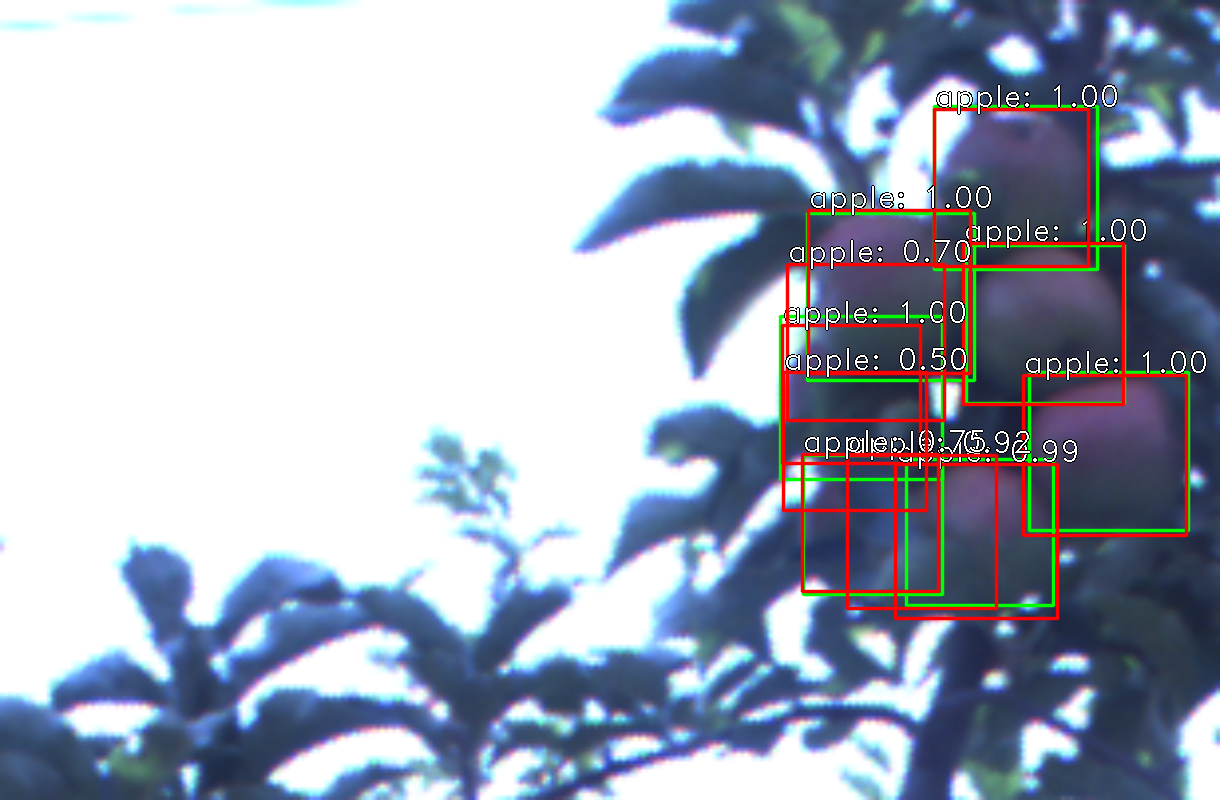
\includegraphics[width=0.38\textwidth]{figures/ch5/fig6_2.png}
    \label{ch5:fig6_2}
  }
  
  \subfigure[$\text{NMS}_{th}=0.3$]{
    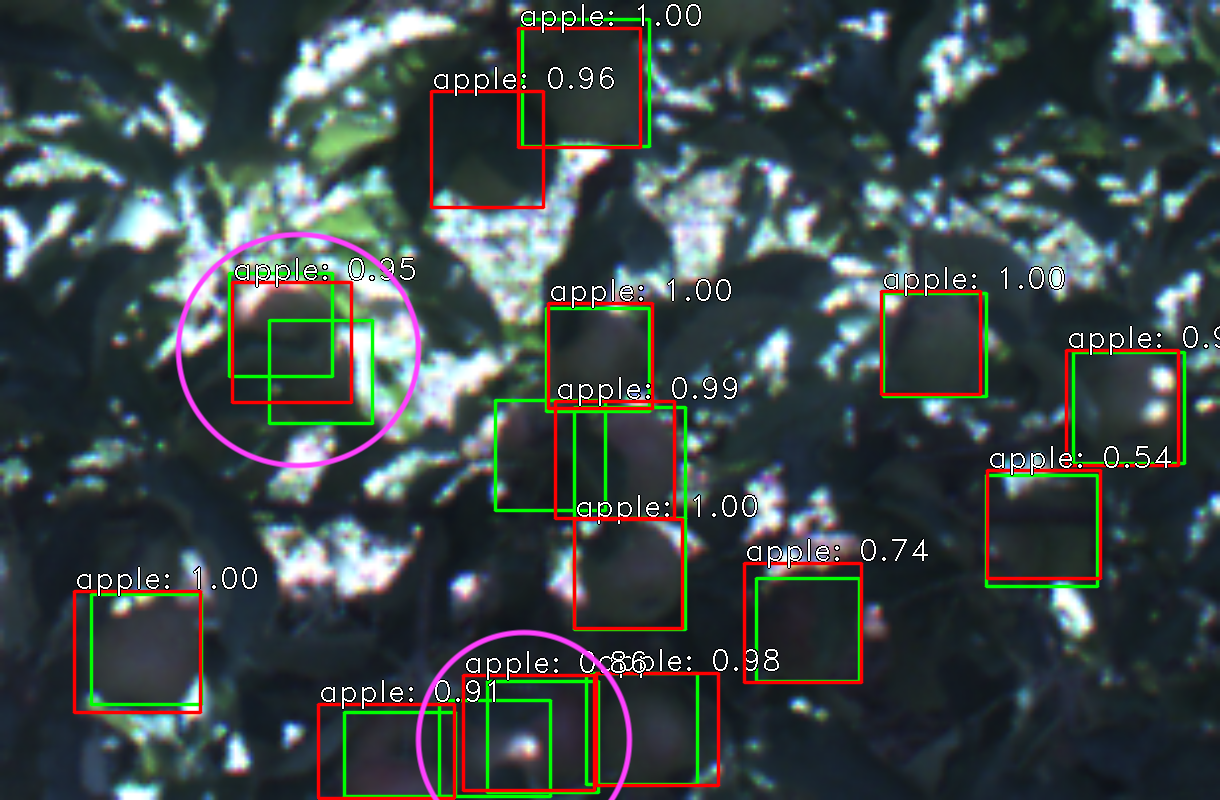
\includegraphics[width=0.38\textwidth]{figures/ch5/fig6_3.png}
    \label{ch5:fig6_3}
  }
  \subfigure[$\text{NMS}_{th}=0.5$]{
    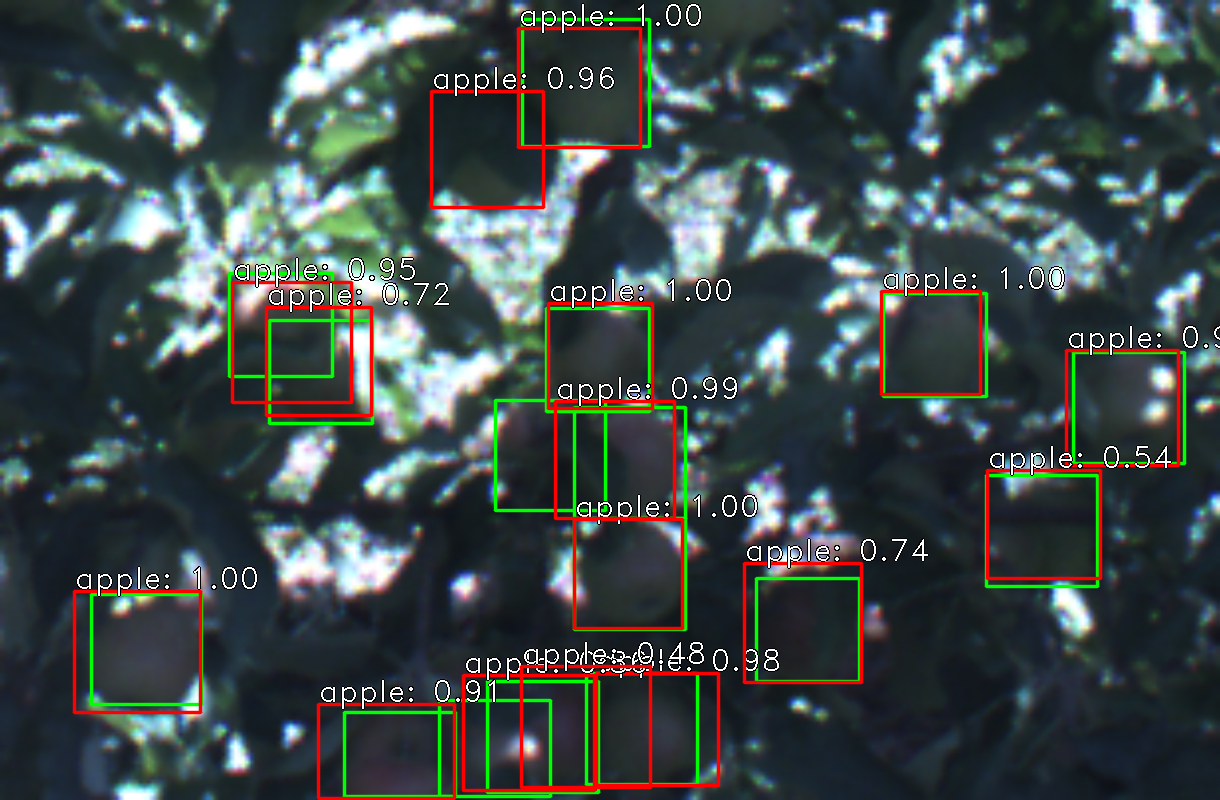
\includegraphics[width=0.38\textwidth]{figures/ch5/fig6_4.png}
    \label{ch5:fig6_4}
  }
  \caption{$\text{NMS}_{th}=0.3$ performs better against clusters (top-left), while fails in occluded fruits such as in the fruits located in the bottom and the far left of the bottom-left image. $\text{NMS}_{th}=0.5$ succeeds in occluded instances, where lower thresholds fail, while fails separating tight clusters resulting in multiple predictions (top-right). Green and red boxes indicate ground truth and predicted annotations respectively.}
  \label{ch5:fig6}
\end{figure}

NMS is responsible for suppressing detections with an overlap over a certain threshold. While it is undoubtedly necessary to avoid multiple detections over the same object, it can be harmful in the fruit detection problem. The detector is fundamentally developed to suppress all predictions with $\text{IoU}\geq\text{NMS}_{th}$ in a query, but one. The dataset contains many fruits in tight clusters or occluded by others; thus the right $\text{NMS}_{th}$ is inextricably linked to the dataset, as it depends on its levels of occlusion between its instances. However, the capability of RetinaNet - $\text{C}_\text{i}\text{Reduced}$ (VGG16) to make precise localisations with an mIoU of 0.835 (\tref{ch5:tab4}), relaxes the $\text{NMS}_{th}$ bounds to the values in \tref{ch5:tab5}. \fref{ch5:fig6} contains sample predictions with different $\text{NMS}_{th}$ values and their impact.

\subsection{Counting}
The dataset does not specify any structure among the trellised trees in the pictures; hence structured yield estimation in the orchard block is impossible. However, $\Delta E$ represents overall count estimates by using the normalised absolute error over the total number of instances in the dataset. $\Delta E$ seems to take smaller values as F1-score increases, giving an unstructured yield estimate for the whole dataset through the total number of predictions. Finally, regarding detector's confidence threshold\footnote{Models' confidence thresholds can be seen in \fref{ch5:fig4}.}, it was optimised to maximise F1-score instead of minimising $\Delta E$.
